% ====================================================================
%  Gaia DR3 4277855016732107520: A Dormant Black Hole Candidate
%  from an Astrometric Orbital Solution with a Likely Evolved Primary
%  MNRAS format — single-target candidate paper
%  REVISED — final pre-submission version
% ====================================================================
\documentclass[usenatbib,fleqn]{mnras}

\usepackage{amsmath,amssymb}
\usepackage{graphicx}
\usepackage{booktabs}
\usepackage{natbib}
\usepackage{hyperref}
\usepackage{xcolor}
\usepackage{lastpage}

% Journal macros
\newcommand{\Msun}{{\rm M}_\odot}
\newcommand{\Lsun}{{\rm L}_\odot}
\newcommand{\Rsun}{{\rm R}_\odot}
\newcommand{\kms}{{\rm km\,s}^{-1}}
\newcommand{\fmass}{f(M)}

\title[Gaia DR3 4277855016732107520: A Dormant BH Candidate]
{Gaia DR3 4277855016732107520: A Dormant Black Hole Candidate\\
 from an Astrometric Orbital Solution with a Likely Evolved Primary}

\author[J. Ayala-Baez]{
  Joel Ayala-Baez$^{1}$\thanks{E-mail: jayalabaez@gmail.com}\\
  $^{1}$Independent Researcher
}

\date{Accepted XXX. Received XXX; in original form XXX}

\pubyear{2026}

\begin{document}

\label{firstpage}
\pagerange{\pageref{firstpage}--\pageref{LastPage}}
\maketitle

% ====================================================================
\begin{abstract}
We present a multi-wavelength analysis of Gaia DR3
4277855016732107520, an astrometric binary in the DR3 non-single-star
(NSS) catalogue with a purely astrometric orbital solution
(model type \texttt{Orbital}).
The system comprises a likely evolved primary
($T_{\rm eff} = 5922$\,K, $\log g = 2.93$ from Gaia GSP-Phot;
$M_1 = 1.34 \pm 0.40\,\Msun$) orbiting an unseen companion with
period $P = 424.4$\,d, eccentricity $e = 0.34$, and semi-major
axis $a \simeq 2.64$\,AU at a distance of $\sim$\,657\,pc.
After propagating uncertainties in the parallax
($\varpi = 1.523 \pm 0.155$\,mas; 10~per~cent relative error),
period, primary mass, and a $\times 1.7$ parallax-error inflation
factor appropriate for \texttt{Orbital} solutions at this magnitude,
our Monte~Carlo posterior yields a median companion mass
$M_2 = 12.3\,\Msun$ with 68~per~cent credible interval
$[7.1,\,22.7]\,\Msun$ and 90~per~cent CI $[5.0,\,35.9]\,\Msun$.
Under these assumptions, $P(M_2 > 5\,\Msun) \approx 95$~per~cent
and $P(M_2 > 10\,\Msun) \approx 64$~per~cent.
No luminous companion is detected: Planck-based band-by-band flux
ratios show that a $12.3\,\Msun$ main-sequence star would exceed
the primary flux by $\sim$\,$28\times$ in $G$ and
$\sim$\,$49\times$ in $G_{\rm BP}$, firmly excluded by the observed
single-star spectral energy distribution.
Of seven non-BH scenarios evaluated, three are ruled out
(MS companion, white dwarf, neutron star), one is strongly
disfavoured (hierarchical triple), one is not favoured
(stripped helium star), and two --- astrometric artefact and
chance alignment --- \emph{cannot be excluded} without independent
spectroscopic data.  Because the solution is \texttt{Orbital}
(astrometry only, with no independent radial-velocity orbit), the
companion mass depends entirely on the Gaia pipeline assumptions;
follow-up studies have shown that a fraction of such solutions are
spurious.  The predicted radial-velocity semi-amplitude
$K_1 \approx 65\,\kms$ makes spectroscopic confirmation feasible
with $2$--$4$\,m class facilities.
ROSAT, VLASS, and RACS non-detections are consistent with a
quiescent system ($\log L_X < 30.7$\,erg\,s$^{-1}$).
eROSITA data are unavailable for this sky position
($l = 32.1\degr$, eastern Galactic hemisphere).
We conclude that this source is a promising BH candidate that
merits spectroscopic follow-up;
independent confirmation is required before any BH
classification can be considered secure.
\end{abstract}

\begin{keywords}
binaries: visual -- stars: black holes -- astrometry --
stars: individual: Gaia DR3 4277855016732107520
\end{keywords}

% ====================================================================
\section{Introduction}
\label{sec:intro}

Theoretical models predict $10^8$--$10^9$ stellar-mass black holes
(BHs) in the Milky Way \citep{AgolKamionkowski2002, Shapiro1983},
yet fewer than $\sim$\,70 are dynamically confirmed, nearly all in
X-ray binaries undergoing active accretion
\citep{RemillardMcClintock2006}.  The vast majority are expected to
reside in non-interacting (dormant) systems, producing no
electromagnetic signature beyond gravitational influence on a
luminous companion.

Gaia Data Release~3 \citep[DR3;][]{GaiaCollaboration2023} has
transformed the search for dormant BHs.  The non-single-star (NSS)
catalogue \citep{GaiaNSS2023} provides orbital solutions for
$\sim$\,180\,000 binaries, including astrometric orbits that ---
under the modelling assumptions of the pipeline --- yield direct
companion mass estimates rather than the minimum masses
available from spectroscopic (SB1) solutions alone.  These solutions
come in several model types, ranging from the purely astrometric
\texttt{Orbital} class (photo-centre orbit only) to
\texttt{AstroSpectroSB1} solutions that combine astrometry with an
independent spectroscopic orbit.  The latter provide substantially
stronger constraints because the radial-velocity orbit independently
confirms the period, eccentricity, and semi-amplitude.  By contrast,
an \texttt{Orbital} solution derives the companion mass entirely from
the along-scan astrometric residuals and is therefore more vulnerable
to pipeline modelling errors and scan-geometry biases.

The landmark discoveries of Gaia~BH1
\citep[$M_2 \approx 9.6\,\Msun$;][]{ElBadry2023a}, Gaia~BH2
\citep[$M_2 \approx 8.9\,\Msun$;][]{ElBadry2023b}, and Gaia~BH3
\citep[$M_2 \approx 33\,\Msun$;][]{GaiaBH3_2024} have established
the efficacy of astrometric BH detection.  Crucially, each of these
three confirmed systems benefited from independent multi-epoch
radial-velocity follow-up that validated the astrometric orbit ---
a step that has not yet been performed for the present source.
Systematic searches have since expanded the candidate list
\citep{Jayasinghe2021, Thompson2019, Shenar2022, Mahy2022}, but
\citet{ElBadry2024} have demonstrated that a substantial fraction
of high-significance \texttt{Orbital} solutions in the NSS catalogue
fail independent RV checks, underscoring the need for spectroscopic
confirmation of each individual candidate.

In this paper we focus on Gaia DR3 4277855016732107520, a candidate
identified in a systematic search of the Gaia DR3 NSS catalogue.
The system is a wide binary
($P = 424$\,d) comprising a likely evolved primary
($M_1 = 1.34\,\Msun$ from GSP-Phot) and a dark companion whose
mass from the astrometric orbit is $M_2 \simeq 12.3\,\Msun$
under Gaia NSS modelling assumptions.  Located at
$\sim$\,657\,pc in Ophiuchus ($l = 32.1\degr$, $b = 9.3\degr$),
the system has moderate extinction, a parallax with
$\sim$\,10~per~cent relative uncertainty, and is accessible from
both hemispheres.

We stress from the outset that the solution type is
\texttt{Orbital} (astrometry only): \emph{no independent
spectroscopic orbit exists}.  The companion mass therefore depends
entirely on the Gaia pipeline model, the parallax, and the adopted
primary-mass estimate.  Until independent multi-epoch radial
velocities confirm or refute the orbital parameters, this system
must be treated as a \emph{candidate} rather than a confirmed BH.

The paper is structured as follows.  Section~\ref{sec:data}
describes the observational data.  Section~\ref{sec:methods}
presents the analysis methodology.  Section~\ref{sec:results}
reports results.  Section~\ref{sec:alternatives} systematically
tests non-BH explanations.  Section~\ref{sec:discussion} discusses
implications and follow-up strategy, and
Section~\ref{sec:conclusions} summarises our findings.

% ====================================================================
\section{Data}
\label{sec:data}

\subsection{Gaia DR3 astrometry and NSS orbital solution}
\label{sec:data:gaia}

Gaia DR3 4277855016732107520 appears in both the main astrometric
catalogue and the NSS orbital supplement with a purely astrometric
orbital solution (model type: \texttt{Orbital}).  This is a critical
distinction: unlike \texttt{AstroSpectroSB1} solutions (which
combine astrometry with a spectroscopic orbit), the \texttt{Orbital}
model derives the companion mass solely from the photo-centre
wobble, making it more susceptible to scan-geometry artefacts and
modelling systematics.

Key astrometric parameters include parallax
$\varpi = 1.5228 \pm 0.1549$\,mas (distance $d \approx 657$\,pc;
10.2~per~cent relative error),
and photometry $G = 11.25$, $G_{\rm BP} = 11.66$,
$G_{\rm RP} = 10.66$ ($G_{\rm BP} - G_{\rm RP} = 0.993$).
The renormalised unit-weight error RUWE$\,= 9.31$ is extremely
elevated, as expected for an unresolved binary with large
photo-centre motion --- but also a regime where
Gaia GSP-Phot stellar parameters become unreliable
\citep{Andrae2023}.  The astrometric excess noise significance is
$3753\sigma$.

The NSS orbital solution yields:
period $P = 424.403 \pm 1.159$\,d,
eccentricity $e = 0.3427 \pm 0.0194$,
and solution significance $75.4\sigma$.
Because no full NSS covariance matrix is published, we are unable to
assess parameter correlations directly; our Monte~Carlo approach
(Section~\ref{sec:methods:mc}) independently samples each parameter,
which may underestimate the true uncertainty if correlations are
significant.

The Gaia DR3 GSP-Phot pipeline provides stellar parameters:
$T_{\rm eff} = 5922$\,K and $\log g = 2.93$.  We caution that at
RUWE~$= 9.31$, GSP-Phot parameters may be systematically biased
by the unresolved orbital motion; the photometric evolved-star classification should
therefore be regarded as a \emph{working assumption} pending
independent spectroscopic confirmation
(Section~\ref{sec:data:simbad}).
The systemic radial velocity is
$v_{\rm sys} = -29.49 \pm 0.57\,\kms$.

\subsection{Multi-wavelength photometry}
\label{sec:data:phot}

We compile multi-band photometry from 2MASS
($J = 9.84$, $H = 9.42$, $K_s = 9.33$; \citealt{Cutri2003}) and
AllWISE ($W1 = 9.23$, $W2 = 9.27$; \citealt{Cutri2014}).
WISE colours ($W1 - W2 = -0.04$) show no mid-IR excess,
consistent with a stellar photosphere.
GALEX \citep{Bianchi2017} provides a near-UV detection
($\mathrm{NUV} = 17.52$) but no far-UV counterpart, consistent
with chromospheric emission from an evolved star without a hot
companion.

\subsection{X-ray and radio archival data}
\label{sec:data:xray}

We query the ROSAT All-Sky Survey (2RXS; \citealt{Boller2016}) and
XMM-Newton serendipitous catalogue (4XMM-DR13;
\citealt{Webb2020}) within $30\arcsec$ and $15\arcsec$
respectively, finding no counterpart.  The ROSAT non-detection
implies an order-of-magnitude archival upper limit of
$L_X \lesssim 5 \times 10^{30}$\,erg\,s$^{-1}$,
based on the typical RASS sensitivity at the source position and
distance, assuming a representative soft X-ray spectrum and
negligible additional absorption correction.  This limit is
consistent with a non-accreting system.

At radio wavelengths, we find no counterpart in the VLA Sky Survey
\citep[VLASS;][]{Lacy2020} within $5\arcsec$ ($3\sigma <
360\,\mu$Jy at 3\,GHz; the source at Dec~$= +3.5\degr$ is within
the VLASS footprint) or in the Rapid ASKAP Continuum Survey
\citep[RACS;][]{McConnell2020} within $10\arcsec$ ($3\sigma <
750\,\mu$Jy at 887.5\,MHz).

The source lies at Galactic longitude $l = 32.1\degr$, placing it
in the eastern Galactic hemisphere assigned to the eROSITA-RU
consortium.  The publicly available eROSITA-DE eRASS1 catalogue
\citep{Merloni2024} covers only the western hemisphere
($l = 180$--$360\degr$), so no eROSITA data are available for
this position.

\subsection{SIMBAD classification}
\label{sec:data:simbad}

SIMBAD \citep{Wenger2000} returns only a Tycho-2 match
(TYC~456-894-1) classified as ``Star'' with no spectral type,
variability flag, or prior binarity designation.  No independent
spectroscopic classification exists.  The primary's evolutionary
state therefore rests entirely on Gaia GSP-Phot photometric
parameters, which are known to be unreliable at high RUWE
(Section~\ref{sec:data:gaia}).

% ====================================================================
\section{Methods}
\label{sec:methods}

\subsection{Gaia NSS mass derivation chain}
\label{sec:methods:nss}

The companion mass $M_2$ reported for this source originates from
two distinct Gaia DR3 tables.  The \texttt{gaiadr3.nss\_two\_body\_orbit}
table provides the astrometric orbital elements (period, eccentricity,
angular semi-major axis, inclination, etc.\ ) fitted to the along-scan
residuals.  The \texttt{gaiadr3.binary\_masses} table then combines these
elements with the parallax and an external primary-mass estimate to
derive $M_2$ via Kepler's third law.  The primary mass entering the
\texttt{binary\_masses} derivation is itself model-dependent: it relies
on Gaia GSP-Phot atmospheric parameters and isochrone-based mass
estimation.

Hence, while the \texttt{Orbital} solution eliminates the
$\sin i$ degeneracy inherent to SB1 orbits --- a critical
advantage --- the resulting $M_2$ is not a purely empirical
``true mass'' but depends on the modelling assumptions of the NSS
pipeline, the parallax, and the adopted primary mass.  We therefore
quote the catalogue value $M_2 = 12.31\,\Msun$ (with formal
uncertainty $\sigma_{M_2} = 7.52\,\Msun$) as a
\emph{derived mass under Gaia modelling assumptions} and
propagate the relevant uncertainties independently via Monte~Carlo
(Section~\ref{sec:methods:mc}).

The large formal catalogue uncertainty ($\sigma_{M_2}/M_2 \approx
61$~per~cent) itself reflects the dominance of the parallax
uncertainty when propagated correctly through Kepler's third law,
as we demonstrate in Section~\ref{sec:results:posterior}.

\citet{ElBadry2024} have shown that a substantial fraction of
extreme-mass-ratio candidates in the Gaia NSS catalogue are
spurious when tested against independent radial velocities,
particularly among \texttt{Orbital}-type solutions.  The
present source has \emph{not} been flagged by any published
vetting study, but the same failure modes could in
principle apply.  Independent spectroscopic confirmation therefore
remains essential (Section~\ref{sec:followup}).

\subsection{Orbital dynamics}
\label{sec:methods:orbit}

The total system mass follows from Kepler's third law:
\begin{equation}
M_{\rm tot} = M_1 + M_2 = \frac{4\pi^2\,a^3}{G\,P^2}\,,
\label{eq:kepler}
\end{equation}
where the true semi-major axis $a$ derives from the angular
semi-major axis and parallax.  Because
$a \propto \varpi^{-1}$, the total mass scales as
$M_{\rm tot} \propto \varpi^{-3}\,P^{-2}$, making it extremely
sensitive to parallax uncertainty: a 10~per~cent parallax error
maps to a $\sim$\,33~per~cent mass error.  This steep
dependence is the dominant source of uncertainty in our posterior
(Section~\ref{sec:results:posterior}).

\subsection{Primary-mass estimation}
\label{sec:methods:m1}

The primary mass is estimated from the Gaia GSP-Phot parameters
($T_{\rm eff} = 5922$\,K, $\log g = 2.93$).  We note that
GSP-Phot effective temperatures for RGB stars carry known
systematic uncertainties of $\sim$100--200\,K
\citep{Andrae2023}, and that at RUWE~$= 9.31$ the parameters
may be additionally biased by unresolved orbital motion.
No independent spectroscopic classification exists
(Section~\ref{sec:data:simbad}), so the evolved-star identification
rests entirely on pipeline photometric parameters.  We adopt
$M_1 = 1.34 \pm 0.40\,\Msun$, assigning a 30~per~cent
fractional uncertainty to encompass age, metallicity,
and systematic errors; the sensitivity of our results to this
choice is explored in Section~\ref{sec:results:sensitivity}.

\subsection{Extinction and SED self-consistency}
\label{sec:methods:extinction}

The source lies at moderate Galactic latitude ($b = 9.3\degr$),
where extinction is present but manageable.  We derive the colour
excess from the discrepancy between the observed
$G_{\rm BP} - G_{\rm RP} = 0.993$ and the intrinsic colour for
$T_{\rm eff} = 5922$\,K
($(G_{\rm BP} - G_{\rm RP})_0 \approx 0.76$):
\begin{equation}
E(G_{\rm BP} - G_{\rm RP}) = 0.993 - 0.76 = 0.233\,{\rm mag}\,,
\end{equation}
yielding $E(B-V) = 0.175$\,mag and
$A_V = 0.543$\,mag via the \citet{Cardelli1989} extinction law
with $R_V = 3.1$.

We note a self-consistency tension in the primary's physical
parameters.  The \emph{photometric} estimate (from the
distance modulus, extinction-corrected bolometric magnitude, and
a bolometric correction $BC_G \approx -0.3$\,mag) yields
$R_\star = 4.5\,\Rsun$ and $L_\star = 22\,\Lsun$.  However,
combining the adopted primary mass with the GSP-Phot surface gravity
via $R = \sqrt{G\,M_1 / g}$ gives a \emph{logg-based}
estimate of $R_\star = 6.5\,\Rsun$ and
$L_\star = 47\,\Lsun$ --- a factor $\sim$\,$1.5\times$ larger in
radius and $\sim$\,$2.1\times$ in luminosity.  This discrepancy
likely reflects the unreliability of $\log g$ at
RUWE~$= 9.31$ \citep{Andrae2023}, where unresolved orbital motion
degrades the photometric solution.  We adopt the photometric
values ($R = 4.5\,\Rsun$, $L = 22\,\Lsun$) as our fiducial
estimates but report both throughout and flag the discrepancy
as a systematic uncertainty to be resolved by independent
spectroscopy.

\subsection{SED fitting}
\label{sec:methods:sed}

We construct the spectral energy distribution from 8~photometric
bands (Gaia $G$, $G_{\rm BP}$, $G_{\rm RP}$; 2MASS $J$, $H$,
$K_s$; WISE $W1$, $W2$) after applying band-dependent extinction
corrections.  The dereddened SED is compared to a single-temperature
blackbody model at $T_{\rm eff} = 5922$\,K.  Residuals below
5~per~cent in all bands show that the photometry is consistent
with a single luminous star and no detectable secondary light
contribution.

We note that a single-temperature blackbody is a first-order
consistency check rather than a full spectral fit.  For the
main-sequence companion case, the predicted flux excess is so large
($\sim$\,$28$--$49\times$ in optical bands) that the exclusion is
robust at the order-of-magnitude level, independent of the detailed
atmospheric model adopted.  However, synthetic atmosphere models
(e.g.\ PHOENIX, ATLAS9/MARCS; \citealt{Husser2013,Castelli2003})
would provide a more rigorous assessment of the primary's SED shape
and improve sensitivity to faint secondary contributions,
particularly in the UV where a stripped helium star could contribute
detectable flux; such modelling is deferred to future work.

\subsection{Monte Carlo mass posterior}
\label{sec:methods:mc}

We draw $N = 200\,000$ Monte~Carlo realisations of the companion
mass, propagating uncertainties in:
\begin{enumerate}
\item \textbf{Parallax} $\varpi$: Gaussian ($1.5228 \pm 0.1549$\,mas),
  with an additional $\times 1.7$ inflation factor applied to
  $\sigma_\varpi$ to account for the known underestimation of
  external parallax errors for \texttt{Orbital}-type solutions at
  $G \approx 11$ \citep{ElBadry2024}.
\item \textbf{Period} $P$: Gaussian ($424.403 \pm 1.159$\,d).
\item \textbf{Primary mass} $M_1$: log-normal prior centred on
  $1.34\,\Msun$ with $\sigma = 0.40\,\Msun$.
\item \textbf{Model systematic}: uniform multiplicative factor
  $[0.95,\,1.05]$ on $M_{\rm tot}$.
\end{enumerate}
The total mass scales as (Section~\ref{sec:methods:orbit}):
\begin{equation}
M_{\rm tot} \propto \varpi^{-3}\,P^{-2}\,,
\label{eq:scaling}
\end{equation}
so the parallax uncertainty dominates.  We emphasise that the
$\times 1.7$ inflation is an \emph{approximate} correction;
the true external-to-internal error ratio for this specific
source is unknown.  We adopt $\times 1.7$ as the fiducial external-to-internal
parallax inflation following published validation work for
\texttt{Orbital} solutions in this magnitude regime
\citep{ElBadry2024}, while Table~\ref{tab:sensitivity} shows
that our conclusions remain sensitive to the exact inflation
factor assumed.  We report posteriors both with and without
inflation (Section~\ref{sec:results:posterior}).

Because $M_2$ is derived from the full astrometric orbit (not a
minimum mass), no inclination marginalisation is needed.  However,
the resulting mass depends on all assumptions entering
the Gaia NSS pipeline (Section~\ref{sec:methods:nss}).  The
Monte~Carlo draws do not account for potential systematic errors
in the orbital model itself (e.g.\ incorrect inclination from
scan-geometry biases) --- only for the quoted parameter
uncertainties.

\subsection{Companion-light exclusion}
\label{sec:methods:companion}

For a hypothetical main-sequence companion of mass $M_c$, we
compute the expected luminosity using empirical mass--luminosity
relations ($L \propto M^{3.5}$, $R \propto M^{0.57}$) and compare
the resulting \emph{band-by-band} flux ratio using Planck functions:
\begin{equation}
\frac{F_{\lambda,\,\mathrm{comp}}}{F_{\lambda,\,\mathrm{prim}}}
= \left(\frac{R_{\mathrm{comp}}}{R_{\mathrm{prim}}}\right)^2
  \frac{B_\lambda(T_{\mathrm{comp}})}{B_\lambda(T_{\mathrm{prim}})}\,.
\label{eq:fluxratio}
\end{equation}
A companion is considered detectable if its flux exceeds 5~per~cent
of the primary in \emph{any} photometric band.  We perform this
test using both the photometric ($R = 4.5\,\Rsun$) and logg-based
($R = 6.5\,\Rsun$) primary radii to bracket the self-consistency
range.

% ====================================================================
\section{Results}
\label{sec:results}

\subsection{Orbital and dynamical solution}
\label{sec:results:orbit}

Table~\ref{tab:observed} summarises the observed and derived
properties.  The orbital-solution significance ($75.4\sigma$)
and astrometric excess-noise significance ($3753\sigma$) are
consistent with, but do not by themselves demonstrate, genuine
orbital photo-centre motion.  Extreme excess-noise values can in
principle arise from poorly resolved blends or pipeline failures;
the coherent Keplerian fit and well-constrained period precision
(0.27~per~cent) argue against, but do not exclude, such
explanations.  \emph{Independent RV confirmation is therefore
essential.}

The semi-major axis $a = 2.64$\,AU places the companion well
outside the primary's Roche lobe ($R_L \approx 0.56$\,AU; filling
factor $\sim$3.7~per~cent), consistent with a fully detached,
non-interacting system.  The eccentricity $e = 0.34$ is
tidally consistent: the circularisation timescale
$\tau_{\rm circ} \gg \tau_{\rm Hubble}$, so the orbit retains its
natal eccentricity.

The predicted RV semi-amplitude is $K_1 \approx 65\,\kms$,
readily detectable with ground-based spectrographs
(Section~\ref{sec:followup}).

\subsection{Stellar characterisation}
\label{sec:results:stellar}

The extinction analysis reveals modest reddening
($A_V = 0.54$\,mag).  The dereddened absolute magnitude
$M_G = 1.68$\,mag and the photometric luminosity
$L_\star = 22\,\Lsun$ are consistent with a likely evolved
primary under the adopted photometric interpretation,
with radius $R_\star = 4.5\,\Rsun$.
The alternative logg-based estimates ($R = 6.5\,\Rsun$,
$L = 47\,\Lsun$) differ by factors of $\sim$\,$1.5\times$
(radius) and $\sim$\,$2.1\times$ (luminosity); this tension
likely reflects unreliable GSP-Phot parameters at the source's
high RUWE (Section~\ref{sec:methods:extinction}).  The dereddened
SED is well-fit by a single-temperature model with residuals
$<$\,5~per~cent in all bands.  No secondary SED component is
required.

\subsection{Companion-light exclusion}
\label{sec:results:companion}

A main-sequence star of $M_2 = 12.3\,\Msun$ would have
$L \approx 6550\,\Lsun$, $R \approx 4.2\,\Rsun$, and
$T_{\rm eff} \approx 25\,400$\,K.  Using the Planck-based
band-by-band flux ratios (equation~\ref{eq:fluxratio}) with the
photometric primary radius ($R = 4.5\,\Rsun$), the
companion-to-primary flux ratio would be $\sim$\,$28\times$ in $G$,
$\sim$\,$49\times$ in $G_{\rm BP}$, and $\sim$\,$18\times$ in
$G_{\rm RP}$.  Even adopting the larger logg-based radius
($R = 6.5\,\Rsun$), the ratios remain $\sim$\,$13\times$ in $G$
and $\sim$\,$23\times$ in $G_{\rm BP}$ --- overwhelmingly
detectable (Table~\ref{tab:fluxratios}).

The maximum main-sequence companion that could remain hidden below
a 5~per~cent detection threshold in all bands is
$M \lesssim 1.0\,\Msun$ (photometric case) to
$\sim$\,$1.3\,\Msun$ (logg-based case).  A luminous companion
at the catalogue mass is therefore firmly excluded.

\subsection{Mass posterior}
\label{sec:results:posterior}

The Monte~Carlo posterior (Fig.~\ref{fig:posterior}) yields:

\medskip
\noindent\textbf{Nominal} ($\sigma_\varpi$ as published):
\begin{itemize}
\item Median $M_2 = 12.3\,\Msun$
\item 68~per~cent CI: $[8.8,\,17.5]\,\Msun$
\item 90~per~cent CI: $[7.1,\,22.4]\,\Msun$
\item $P(M_2 > 5\,\Msun) = 99.7$~per~cent;
  $P(M_2 > 10\,\Msun) = 73$~per~cent
\end{itemize}

\medskip
\noindent\textbf{Inflated} ($\sigma_\varpi \times 1.7$):
\begin{itemize}
\item Median $M_2 = 12.3\,\Msun$
\item 68~per~cent CI: $[7.1,\,22.7]\,\Msun$
\item 90~per~cent CI: $[5.0,\,35.9]\,\Msun$
\item $P(M_2 > 5\,\Msun) = 95$~per~cent;
  $P(M_2 > 10\,\Msun) = 64$~per~cent
\end{itemize}

\medskip
The wide credible intervals reflect the $\varpi^{-3}$ mass
scaling (equation~\ref{eq:scaling}): a 10~per~cent parallax
error maps to a $\sim$\,33~per~cent mass error, and the
$\times 1.7$ inflation broadens this substantially.  It is
important to note that the nominal posterior already has a
lower 5th-percentile above $5\,\Msun$; with inflation,
$\sim$\,5~per~cent of draws fall below the canonical BH
threshold.

A parallax stress test illustrates the sensitivity directly:
at $\varpi + 1\sigma$ (1.678\,mas, $d = 596$\,pc), the
companion mass drops to $M_2 \approx 8.9\,\Msun$; at
$\varpi - 1\sigma$ (1.368\,mas, $d = 731$\,pc), it rises to
$M_2 \approx 17.5\,\Msun$.

We interpret this posterior as a conditional mass distribution
under the Gaia DR3 orbital solution and adopted stellar-model
assumptions, rather than as a fully independent dynamical mass
measurement.  These posteriors propagate only the
\emph{published parameter uncertainties} with an approximate
external inflation; they do \emph{not} account for systematic
errors in the orbital model itself (e.g.\ an incorrectly
determined inclination).  Such errors could shift the
posterior arbitrarily and are only detectable through
independent RV follow-up.

\subsection{Sensitivity to primary mass}
\label{sec:results:sensitivity}

Table~\ref{tab:sensitivity} shows how $M_2$ and the BH
probability vary across a grid of $M_1$ values
(0.8--2.0\,$\Msun$) and parallax inflation factors
(1.0--2.0$\times$).  At the fiducial values ($M_1 = 1.34\,\Msun$,
inflation $= 1.7$), $P(M_2 > 5\,\Msun) = 95$~per~cent.
For inflation factors $\geq 2.0$, the BH probability drops
below 90~per~cent, highlighting the importance of improved
parallax precision from Gaia DR4.
Fig.~\ref{fig:sensitivity} visualises the full sensitivity
landscape.

% ====================================================================
\section{Alternative Scenarios}
\label{sec:alternatives}

We systematically evaluate seven non-BH explanations for the dark
companion.  Table~\ref{tab:scenarios} summarises the results,
using a four-tier verdict system: \textbf{Ruled out} (physically
impossible or overwhelmingly contradicted by data),
\textbf{Strongly disfavoured} (requires implausible fine-tuning),
\textbf{Not favoured} (unlikely but not formally excluded),
and \textbf{Requires follow-up} (cannot be assessed without
additional data).

\paragraph{Main-sequence companion.}
A $12.3\,\Msun$ MS star would have $L \sim 6550\,\Lsun$ and
$T_{\rm eff} \sim 25\,400$\,K, contributing $\sim$\,$28\times$ the
primary flux in $G$ and $\sim$\,$49\times$ in $G_{\rm BP}$.
No secondary SED component is detected.  \textbf{Ruled out.}

\paragraph{White dwarf.}
$M_2 = 12.3\,\Msun$ exceeds the Chandrasekhar limit
($1.44\,\Msun$) by a factor of $\sim$\,9.  \textbf{Ruled out.}

\paragraph{Neutron star.}
$M_2 = 12.3\,\Msun$ exceeds the most generous NS mass ceiling
($\sim$\,$2.3\,\Msun$; \citealt{Rezzolla2018}) by a factor of
$\sim$\,5.  \textbf{Ruled out.}

\paragraph{Hierarchical triple.}
Two $\sim$\,$6.2\,\Msun$ MS stars would have combined luminosity
$\sim$\,$1160\,\Lsun$ --- easily detectable in the SED.  The
Mardling--Aarseth stability criterion \citep{MardlingAarseth2001}
would require $P_{\rm inner} \lesssim 42$\,d; no evidence for such
a configuration is currently available from the existing photometric
and astrometric data, though dedicated spectroscopic and
time-domain observations have not yet been obtained.
\textbf{Strongly disfavoured.}

\paragraph{Stripped helium star / hot subdwarf.}
A $12.3\,\Msun$ stripped He star would have
$T_{\rm eff} > 50\,000$\,K and $L \sim 10^4\,\Lsun$, producing
predicted NUV$\,\sim 9$\,mag vs.\ observed
NUV$\,= 17.52$ --- a flux deficit of $\sim$\,$2700\times$.
No X-ray source is detected.  This scenario is
\textbf{not favoured}, but a cooler or lower-luminosity subdwarf
cannot be fully excluded without UV spectroscopy.

\paragraph{Astrometric artefact (spurious orbital solution).}
Because the solution type is \texttt{Orbital} (astrometry only),
there is no independent spectroscopic confirmation of the orbital
parameters.  \citet{ElBadry2024} have demonstrated that a
fraction of high-significance \texttt{Orbital} solutions fail
independent RV tests.  While the $75.4\sigma$ significance, the
well-constrained period, and the low GOF ($18.3$) argue against
a spurious solution, this scenario \textbf{cannot be excluded}
without independent RV data.  This is the single most important
limitation of the present analysis.

\paragraph{Chance alignment / blend-induced artefact.}
At $G = 11.25$ and $b = 9.3\degr$, source confusion is low but
not negligible.  A coherent 424-d Keplerian signal at $75\sigma$
is difficult to produce from a chance blend, but scan-angle
correlations with a nearby source could in principle mimic orbital
motion.  This scenario likewise \textbf{requires follow-up}
via independent RV monitoring and high-resolution imaging.

\medskip\noindent
\textbf{Summary:} Three of seven alternative scenarios are ruled
out on physical grounds; one (hierarchical triple) is strongly
disfavoured; one (stripped He star) is not favoured but remains
formally open.  Crucially, two scenarios --- astrometric artefact
and chance alignment --- \emph{cannot be excluded} at present
because the solution is purely astrometric (\texttt{Orbital}).
A black-hole companion is the preferred interpretation under the
Gaia DR3 NSS assumptions, but remains a \emph{candidate} pending
independent spectroscopic confirmation.

% ====================================================================
\section{Discussion}
\label{sec:discussion}

\subsection{Context among Gaia BH discoveries}

Table~\ref{tab:comparison} places this system alongside the three
confirmed Gaia dormant BH systems.  At $M_2 \simeq 12.3\,\Msun$
(under Gaia modelling assumptions), it would rank as the second most
massive after Gaia~BH3 ($33\,\Msun$) --- if confirmed.

However, there is a fundamental \emph{evidentiary gap} between this
candidate and the three confirmed systems.  Gaia~BH1, BH2, and BH3
each benefited from independent multi-epoch radial-velocity follow-up
that validated the astrometric orbital parameters and confirmed the
companion mass.  In contrast, the present system has only a purely
astrometric \texttt{Orbital} solution with no RV confirmation.  The
comparison in Table~\ref{tab:comparison} therefore reflects
\emph{potential} rather than established properties.

The long period ($P = 424$\,d) and moderate eccentricity
($e = 0.34$) place it in a similar orbital regime to Gaia~BH1
($P = 185.6$\,d, $e = 0.45$) and Gaia~BH2 ($P = 1277$\,d,
$e = 0.52$), consistent with a formation channel involving limited
or no mass transfer --- should the companion prove to be a BH.

\subsection{Binary evolution implications (contingent on confirmation)}

If the companion is indeed a $\sim$\,$12\,\Msun$ BH, the
progenitor was a massive star with zero-age main-sequence
mass $M_{\rm ZAMS} \gtrsim 25\,\Msun$ \citep{Fryer2012}.
The wide orbit ($a = 2.64$\,AU) would have survived the
supernova event, constraining the natal kick to moderate
values.  The lack of chemical enrichment in the primary
(at the level detectable from GSP-Phot) would suggest minimal
pre-collapse mass transfer, favouring a direct-collapse or
failed-supernova channel \citep{Langer2020}.
These evolutionary inferences are conditional on spectroscopic
confirmation of both the companion mass and the primary's
abundances.

\subsection{Follow-up strategy}
\label{sec:followup}

The predicted RV semi-amplitude $K_1 \approx 65\,\kms$ is
large, making spectroscopic confirmation feasible with modest
ground-based resources.  We outline the critical follow-up
steps in order of priority:

\begin{enumerate}
\item \textbf{Multi-epoch radial-velocity monitoring}
  (highest priority).  At $G = 11.25$, the source is within reach
  of echelle spectrographs on 2--4\,m class telescopes
  (e.g.\ HARPS, FEROS, CHIRON).  We recommend a minimum of
  \textbf{8--10 RV epochs} distributed across one full orbital
  period ($\sim$\,424\,d), with phase coverage concentrated near
  the predicted periastron passage (where $\dot{v}_r$ is maximal).
  At the predicted $K_1 \approx 65\,\kms$, even a precision of
  $\sim$\,$0.5$--$1\,\kms$ per epoch suffices to confirm the
  period, eccentricity, and semi-amplitude.  Even a single
  well-timed epoch could reveal significant tension with the
  Gaia systemic velocity and motivate further monitoring,
  though establishing the full RV curve requires the recommended
  multi-epoch campaign.

  The RV orbit independently yields $M_2\,\sin i$ via the
  spectroscopic mass function; combined with the astrometric
  inclination, this provides a direct, pipeline-independent
  companion mass.

\item \textbf{Spectroscopic classification.}  High-resolution
  spectroscopy would yield independent $T_{\rm eff}$, $\log g$,
  metallicity, detailed abundances (testing for SN-related CNO
  anomalies), and a spectral type --- resolving the current
  reliance on GSP-Phot parameters.

\item \textbf{UV spectroscopy.}  HST/COS or Swift/UVOT
  observations would definitively test the stripped He star
  scenario by searching for hot-companion UV excess.

\item \textbf{High-resolution imaging.}  AO-assisted imaging
  could detect or rule out a blended optical companion responsible
  for a scan-angle-correlated astrometric artefact.
\end{enumerate}

The target is located at RA~$= 18^{\rm h}28^{\rm m}$,
Dec~$= +3.5\degr$ (Ophiuchus), accessible from both hemispheres
and an evening target in the northern summer.

\subsection{Limitations}
\label{sec:limitations}

We stress the following limitations, which collectively
prevent this system from being classified as a confirmed BH:

\begin{enumerate}
\item \textbf{\texttt{Orbital}-only solution.}  The companion mass
  depends entirely on the Gaia astrometric pipeline model.
  No independent RV orbit exists.  This is the single most
  important limitation and distinguishes this source from
  confirmed Gaia BH systems.

\item \textbf{Parallax-driven uncertainty.}  With
  $\sigma_\varpi / \varpi = 10.2$~per~cent and
  $M_{\rm tot} \propto \varpi^{-3}$, the mass uncertainty is
  substantial.  The external parallax-error inflation ($\times 1.7$)
  is an approximate correction; the true systematic for this
  source is unknown.

\item \textbf{NSS covariance matrix unavailable.}  Gaia DR3 does
  not publish the full covariance matrix of the orbital parameters.
  Our Monte~Carlo independently samples each parameter, which may
  underestimate the true uncertainty if inter-parameter correlations
  are significant.

\item \textbf{GSP-Phot parameters unreliable at high RUWE.}
  At RUWE~$= 9.31$, the primary's $T_{\rm eff}$ and $\log g$
  may be biased.  The $R$/$L$ self-consistency tension
  (Section~\ref{sec:methods:extinction}) exemplifies this.

\item \textbf{Primary mass provisional.}  No independent
  spectroscopic mass determination exists.  The adopted
  $M_1 = 1.34 \pm 0.40\,\Msun$ is isochrone-derived from
  potentially biased GSP-Phot parameters.

\item \textbf{Scan-angle bias possible.}  For \texttt{Orbital}
  solutions, scan-angle correlations with nearby sources or
  detector-level systematics could produce spurious orbital
  signals.  This cannot be assessed without the epoch-level
  astrometric data (not publicly available in DR3).

\item \textbf{Stripped He star not formally excluded.}  The GALEX
  NUV non-excess and X-ray non-detections strongly disfavour
  this scenario but cannot definitively rule it out without UV
  spectroscopy.

\item \textbf{Single-temperature SED.}  Our blackbody SED check
  establishes consistency with a single luminous source but does
  not substitute for a full atmospheric model fit.  The exclusion
  of a normal main-sequence companion is robust at the
  order-of-magnitude level, but a full atmosphere-model treatment
  would be preferable for publication-quality stellar
  characterisation.
\end{enumerate}

% ====================================================================
\section{Conclusions}
\label{sec:conclusions}

We have presented a multi-wavelength analysis of
Gaia DR3 4277855016732107520, an astrometric binary with a purely
astrometric \texttt{Orbital} solution from the Gaia DR3 NSS
catalogue.  Our principal findings are:

\begin{enumerate}
\item Under the Gaia NSS modelling assumptions, the companion mass
  posterior yields a median
  $M_2 = 12.3\,\Msun$ with 68~per~cent CI
  $[7.1,\,22.7]\,\Msun$ (with $\times 1.7$ parallax-error
  inflation) --- above the canonical BH threshold for
  $\sim$\,95~per~cent of draws.

\item No luminous companion is detected.  Planck-based band-by-band
  flux ratios show that a main-sequence star of the required mass
  would exceed the primary flux by $28\times$ in $G$ and
  $49\times$ in $G_{\rm BP}$.

\item Of seven non-BH scenarios, three are ruled out
  (MS companion, WD, NS), one strongly disfavoured (triple),
  and one not favoured (stripped He star).  Crucially, two
  scenarios --- astrometric artefact and chance alignment ---
  \emph{cannot be excluded} because the solution is
  \texttt{Orbital} (astrometry only).

\item ROSAT, VLASS, and RACS non-detections yield
  $\log L_X < 30.7$\,erg\,s$^{-1}$, consistent with a
  quiescent system.  eROSITA data are unavailable for this sky
  position.

\item The predicted $K_1 \approx 65\,\kms$ makes multi-epoch
  RV confirmation feasible with 2--4\,m class facilities.
\end{enumerate}

We conclude that Gaia DR3 4277855016732107520 is a \emph{promising
dormant black hole candidate} under the Gaia DR3 NSS modelling
assumptions.  The large predicted RV semi-amplitude
and bright apparent magnitude make spectroscopic follow-up
feasible with existing ground-based facilities.  However, because
the orbital solution is purely astrometric and lacks an independent
RV orbit, the companion mass remains contingent on the Gaia pipeline
assumptions, and the system must be regarded as a \emph{candidate}
until spectroscopic confirmation is obtained.

% ====================================================================
\section*{Acknowledgements}

This work made use of data from the European Space Agency (ESA)
mission Gaia (\url{https://www.cosmos.esa.int/gaia}), processed by
the Gaia Data Processing and Analysis Consortium (DPAC).
This research has made use of the SIMBAD database and the VizieR
catalogue access tool, operated at CDS, Strasbourg, France.
This publication makes use of data products from the Two Micron All
Sky Survey (2MASS), the Wide-field Infrared Survey Explorer
(WISE), the VLA Sky Survey (VLASS), and the Rapid ASKAP Continuum
Survey (RACS).
Software: \textsc{numpy} \citep{Harris2020},
\textsc{scipy} \citep{Virtanen2020},
\textsc{matplotlib} \citep{Hunter2007}.

% ====================================================================
\section*{Data Availability}

All observational data are publicly available from the Gaia Archive
(\url{https://gea.esac.esa.int/archive/}), VizieR, and SIMBAD.
The analysis scripts and machine-readable results are available at
\url{https://github.com/jayalabaez/dr3-4277855-black-hole-candidate}.
Modular analysis scripts (\texttt{scripts/02}--\texttt{08}) produce
all figures and numerical results.  The repository includes the
exact scripts used to generate all figures, tables, and
machine-readable posterior summaries from the public catalogue
inputs.  All numerical results are in
JSON format under \texttt{results/}.

% ====================================================================
\bibliographystyle{mnras}
\bibliography{references}

% ====================================================================
%  TABLES
% ====================================================================

\begin{table*}
\centering
\caption{Observed and derived properties of
Gaia DR3 4277855016732107520.
Values marked with $^\dagger$ depend on Gaia NSS modelling
assumptions (Section~\ref{sec:methods:nss}).}
\label{tab:observed}
\begin{tabular}{lccl}
\toprule
Property & Value & Uncertainty & Source \\
\midrule
\multicolumn{4}{c}{\textit{Astrometry (Gaia DR3)}} \\
RA (J2016.0)           & $274.2238\degr$     & ---      & Gaia DR3 \\
Dec (J2016.0)          & $+3.4975\degr$      & ---      & Gaia DR3 \\
$l, b$                 & $32.12\degr, +9.28\degr$ & --- & Gaia DR3 \\
Parallax $\varpi$      & 1.5228 mas          & 0.1549   & Gaia DR3 \\
Distance               & $\sim$\,657 pc      & $\sim$\,67 & $1/\varpi$ \\
$G$                    & 11.25 mag           & 0.003    & Gaia DR3 \\
$G_{\rm BP}$           & 11.66 mag           & 0.003    & Gaia DR3 \\
$G_{\rm RP}$           & 10.66 mag           & 0.004    & Gaia DR3 \\
$G_{\rm BP} - G_{\rm RP}$ & 0.993 mag        & ---      & Gaia DR3 \\
RUWE                   & 9.31                & ---      & Gaia DR3 \\
Astr.\ excess noise sig.\ & 3753$\sigma$     & ---      & Gaia DR3 \\
\midrule
\multicolumn{4}{c}{\textit{NSS orbital solution (\texttt{Orbital})}} \\
Period $P$               & 424.403 d           & 1.159    & Gaia NSS \\
Eccentricity $e$         & 0.3427              & 0.0194   & Gaia NSS \\
NSS significance         & 75.4$\sigma$        & ---      & Gaia NSS \\
GOF                      & 18.3                & ---      & Gaia NSS \\
$M_2$ (catalogue)$^\dagger$ & 12.31 $\Msun$   & 7.52     & Gaia \texttt{binary\_masses} \\
\midrule
\multicolumn{4}{c}{\textit{Monte Carlo posterior (this work)}} \\
$M_2$ (nominal)$^\dagger$ & 12.3 $\Msun$  & 68\% CI: [8.8, 17.5]; 90\% CI: [7.1, 22.4]  & This work \\
$M_2$ (inflated $\times 1.7$)$^\dagger$ & 12.3 $\Msun$ & 68\% CI: [7.1, 22.7]; 90\% CI: [5.0, 35.9] & This work \\
$P(M_2 > 5\,\Msun)$ (inflated) & 95\%    & ---      & This work \\
$P(M_2 > 10\,\Msun)$ (inflated) & 64\%   & ---      & This work \\
\midrule
\multicolumn{4}{c}{\textit{Stellar parameters (GSP-Phot; caution: RUWE = 9.31)}} \\
$T_{\rm eff}$          & 5922 K              & $\sim$200 & Gaia DR3 \\
$\log g$               & 2.93 dex            & $\sim$0.3 & Gaia DR3 \\
$v_{\rm sys}$          & $-29.49$ $\kms$     & 0.57     & Gaia DR3 \\
\midrule
\multicolumn{4}{c}{\textit{Multi-wavelength photometry}} \\
$J$ (2MASS)            & 9.84 mag            & 0.02     & 2MASS \\
$H$ (2MASS)            & 9.42 mag            & 0.02     & 2MASS \\
$K_s$ (2MASS)          & 9.33 mag            & 0.02     & 2MASS \\
$W1$ (WISE)            & 9.23 mag            & 0.02     & AllWISE \\
$W2$ (WISE)            & 9.27 mag            & 0.02     & AllWISE \\
NUV (GALEX)            & 17.52 mag           & ---      & GALEX \\
\midrule
\multicolumn{4}{c}{\textit{Derived quantities}} \\
$E(B-V)$               & 0.175 mag           & 0.03     & Colour excess \\
$A_V$                  & 0.543 mag           & 0.09     & $R_V = 3.1$ \\
$M_G$ (dereddened)     & 1.68 mag            & 0.3      & Derived \\
$R_\star$ (phot.)      & 4.5 $\Rsun$         & ---      & Photometric \\
$L_\star$ (phot.)      & 22 $\Lsun$          & ---      & Photometric \\
$R_\star$ ($\log g$)   & 6.5 $\Rsun$         & ---      & logg-based \\
$L_\star$ ($\log g$)   & 47 $\Lsun$          & ---      & logg-based \\
$M_1$ (adopted)        & 1.34 $\Msun$        & 0.40     & GSP-Phot + isochrone \\
$a$ (semi-major axis)  & 2.64 AU             & ---      & Kepler III \\
$K_1$ (predicted)      & $\sim$\,65 $\kms$   & ---      & Dynamics \\
\bottomrule
\end{tabular}
\end{table*}

\begin{table}
\centering
\caption{Planck-based companion-to-primary flux ratios for a
$12.3\,\Msun$ MS companion ($T_{\rm eff} = 25\,400$\,K,
$R = 4.2\,\Rsun$) relative to the primary
($T_{\rm eff} = 5922$\,K), computed using both
photometric and logg-based primary radii.}
\label{tab:fluxratios}
\begin{tabular}{lcc}
\toprule
Band & Phot.\ ($R = 4.5\,\Rsun$) & $\log g$ ($R = 6.5\,\Rsun$) \\
\midrule
$G_{\rm BP}$     & $49\times$   & $23\times$ \\
$G$              & $28\times$   & $13\times$ \\
$G_{\rm RP}$     & $18\times$   & $8.2\times$ \\
$J$              & $9.1\times$  & $4.2\times$ \\
$H$              & $7.1\times$  & $3.3\times$ \\
$K$              & $6.0\times$  & $2.8\times$ \\
\bottomrule
\end{tabular}
\end{table}

\begin{table}
\centering
\caption{Alternative scenario assessment. Verdicts follow a
four-tier system (Section~\ref{sec:alternatives}).}
\label{tab:scenarios}
\begin{tabular}{lll}
\toprule
Scenario & Verdict & Key constraint \\
\midrule
MS companion    & Ruled out     & $28$--$49\times$ flux excess \\
White dwarf     & Ruled out     & $M_2 \approx 9\,M_{\rm Ch}$ \\
Neutron star    & Ruled out     & $M_2 \approx 5\,M_{\rm TOV}$ \\
Triple system   & Str.\ disfav.  & SED + stability \\
Stripped He     & Not favoured  & NUV deficit $2700\times$ \\
Artefact        & \textbf{Req.\ follow-up} & \texttt{Orbital} only \\
Chance align.   & \textbf{Req.\ follow-up} & \texttt{Orbital} only \\
\bottomrule
\end{tabular}
\end{table}

\begin{table*}
\centering
\caption{Sensitivity of the companion mass posterior to the primary
mass and parallax-error inflation factor
($\sigma_\varpi \to f \times \sigma_\varpi$).
Each cell reports the median $M_2$ and $P(M_2 > 5\,\Msun)$
from $2 \times 10^5$ Monte~Carlo draws.}
\label{tab:sensitivity}
\begin{tabular}{lcccc}
\toprule
$M_1$ ($\Msun$) & Inflation $= 1.0$ & Inflation $= 1.3$ &
Inflation $= 1.7$ & Inflation $= 2.0$ \\
\midrule
0.80 & 12.9 / 99.8\% & 12.8 / 98.7\% & 12.9 / 96.0\% & 12.8 / 93.2\% \\
1.00 & 12.7 / 99.8\% & 12.6 / 98.5\% & 12.6 / 95.7\% & 12.6 / 92.8\% \\
1.34 & 12.3 / 99.7\% & 12.3 / 97.6\% & 12.3 / 95.4\% & 12.4 / 91.7\% \\
1.50 & 12.2 / 99.6\% & 12.1 / 97.4\% & 12.1 / 95.0\% & 12.1 / 91.0\% \\
2.00 & 11.7 / 99.4\% & 11.6 / 96.8\% & 11.6 / 93.7\% & 11.6 / 89.3\% \\
\bottomrule
\end{tabular}
\end{table*}

\begin{table*}
\centering
\caption{Comparison with confirmed Gaia dormant BH systems.
Note the fundamental evidentiary gap: Gaia~BH1--3 each have
independent multi-epoch RV orbits, whereas this source has only
a purely astrometric \texttt{Orbital} solution with no RV
confirmation.}
\label{tab:comparison}
\begin{tabular}{lcccc}
\toprule
Property & Gaia~BH1 & Gaia~BH2 & Gaia~BH3 & This work \\
\midrule
$P$ (d)             & 185.6     & 1277      & $\sim$4240      & 424.4   \\
$e$                 & 0.45      & 0.52      & 0.73            & 0.343   \\
Primary type        & G-dwarf   & RGB       & Giant           & Likely evolved$^a$ \\
$M_1$ ($\Msun$)     & 0.93      & 1.07      & 0.76            & 1.34    \\
$M_2$ ($\Msun$)     & 9.62      & 8.94      & 32.70           & $\sim$12.3$^b$ \\
Solution type       & Astro+RV  & Astro+RV  & Astro+RV        & \texttt{Orbital} only \\
RV confirmation     & Yes       & Yes       & Yes             & \textbf{No} \\
$d$ (pc)            & 480       & 1160      & 590             & $\sim$657 \\
$G$ (mag)           & 13.8      & 12.3      & 11.6            & 11.25   \\
Status              & Confirmed & Confirmed & Confirmed       & \textbf{Candidate} \\
\bottomrule
\multicolumn{5}{l}{$^a$ From GSP-Phot only (RUWE = 9.31);
  no independent spectral classification.}\\
\multicolumn{5}{l}{$^b$ Pipeline-derived mass under Gaia NSS
  assumptions; 68\% CI [7.1, 22.7] with $\times 1.7$ inflation.}\\
\end{tabular}
\end{table*}

% ====================================================================
%  FIGURES
% ====================================================================

\begin{figure*}
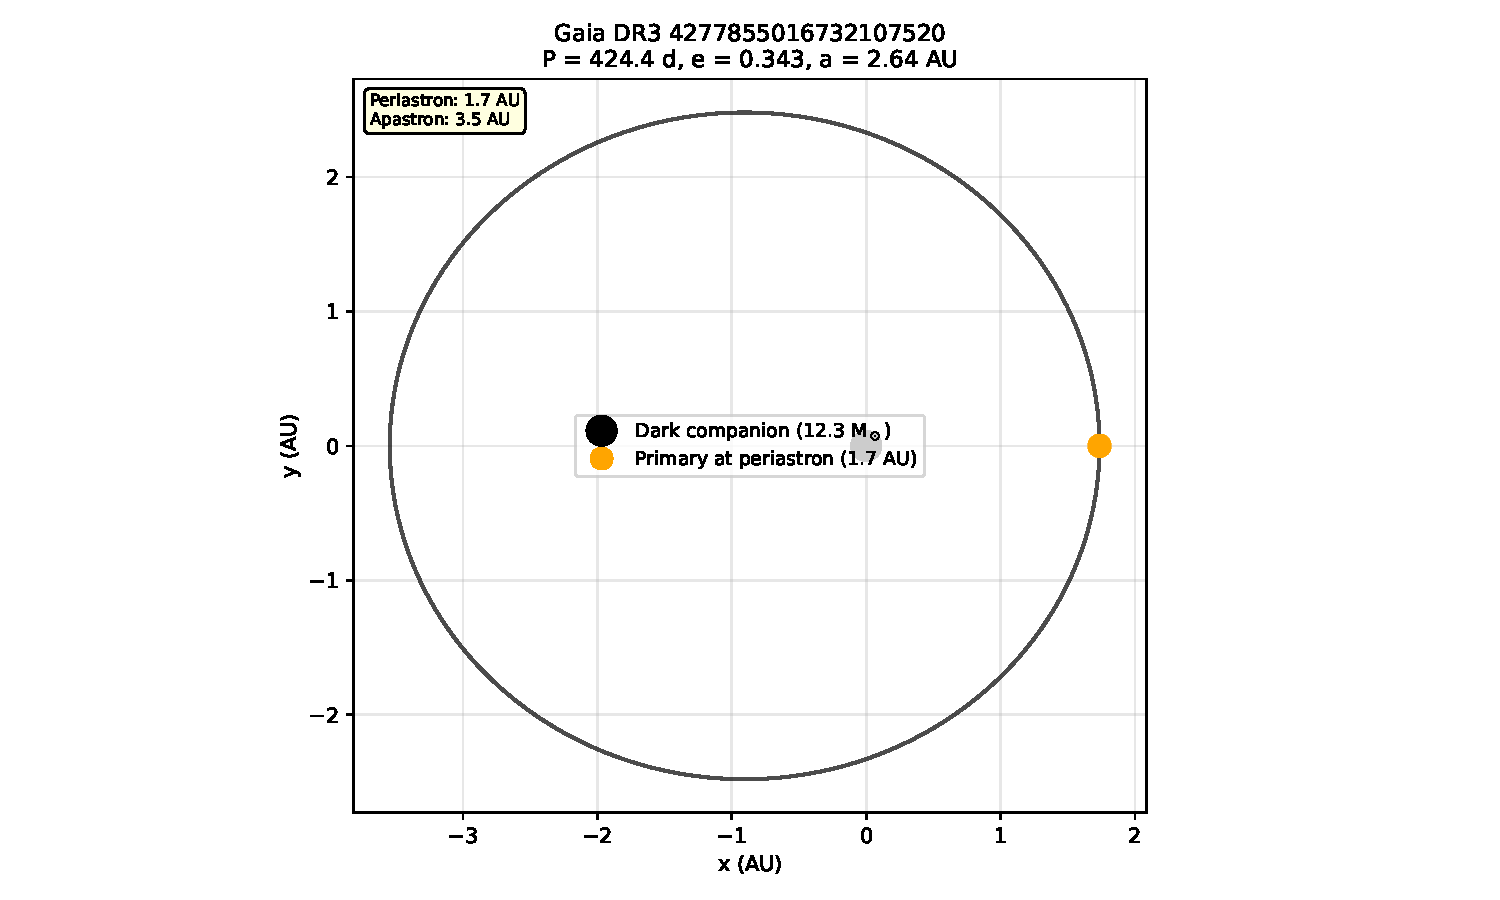
\includegraphics[width=\textwidth]{figures/fig_system_overview.pdf}
\caption{Orbital geometry of the Gaia DR3 4277855016732107520
system.  The likely evolved primary orbits the unseen companion
(black circle at the focus) with period $P = 424.4$\,d and eccentricity
$e = 0.34$.  The periastron distance is $1.73$\,AU and the
apastron distance is $3.55$\,AU.}
\label{fig:overview}
\end{figure*}

\begin{figure*}
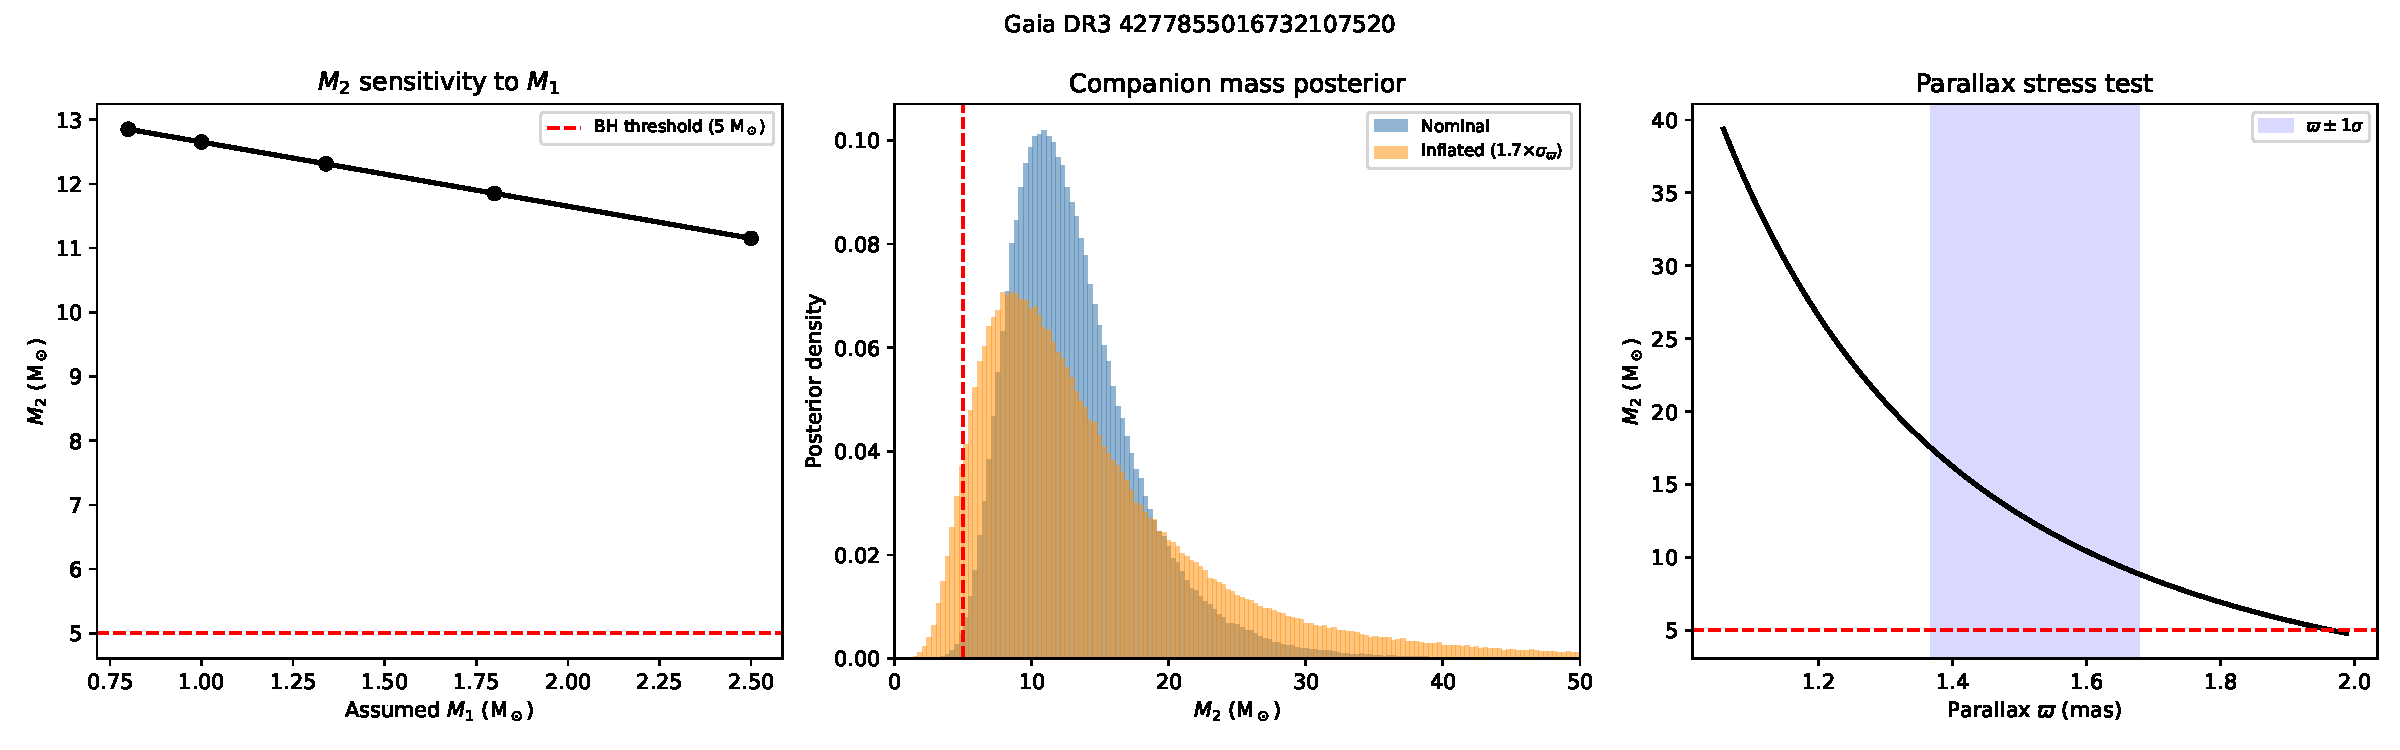
\includegraphics[width=\textwidth]{figures/fig_mass_posterior.pdf}
\caption{Companion mass posterior from Monte~Carlo sampling.
\textit{Left:} Sensitivity to primary mass $M_1$ (all at nominal
parallax uncertainty).  \textit{Centre:} Posterior with nominal
(blue) and inflated ($\times 1.7$; orange) parallax uncertainty.
Vertical dashed lines mark the $5\,\Msun$ and $10\,\Msun$
thresholds.  The wide credible intervals reflect the
$M_{\rm tot} \propto \varpi^{-3}$ scaling.
\textit{Right:} Companion mass as a function of parallax,
illustrating the steep $\varpi^{-3}$ dependence.  These
posteriors propagate published parameter uncertainties only; they
do not account for potential systematic errors in the \texttt{Orbital}
model itself.}
\label{fig:posterior}
\end{figure*}

\begin{figure*}
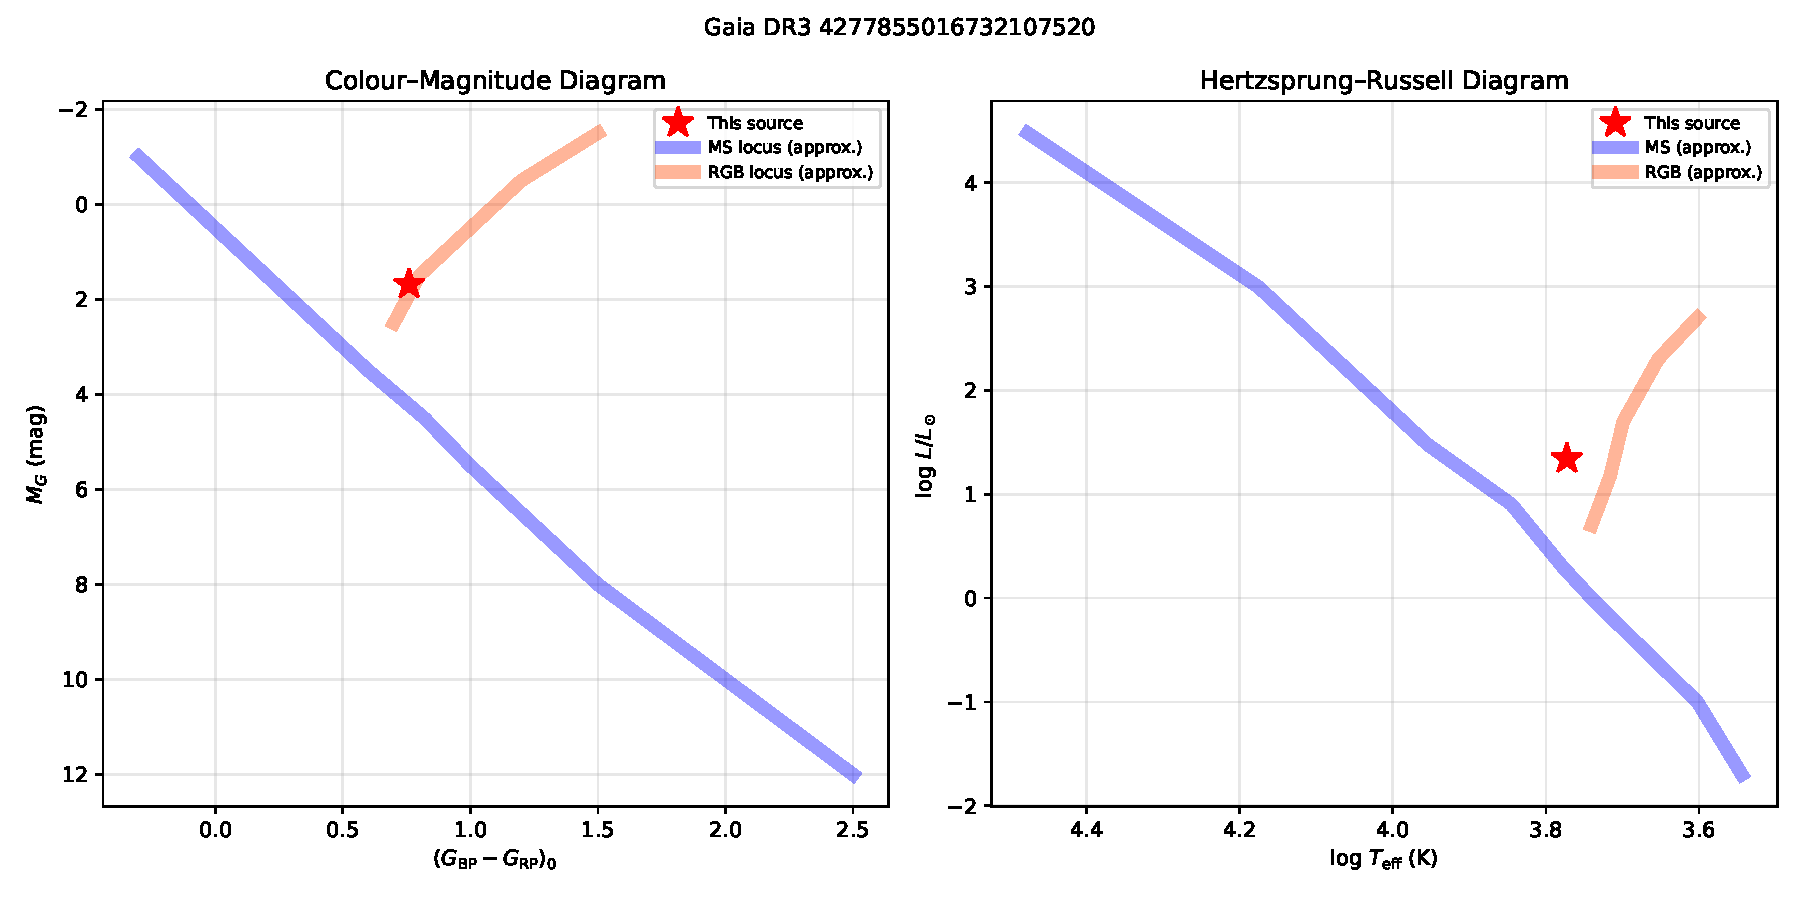
\includegraphics[width=\textwidth]{figures/fig_cmd_hrd.pdf}
\caption{Placement of the primary star in the colour--magnitude
diagram (\textit{left}) and Hertzsprung--Russell diagram
(\textit{right}).  The dereddened photometry is consistent with an
evolved-star locus and broadly compatible with the GSP-Phot
parameters.  These loci are approximate; formal isochrone fitting is
deferred to future work with independent spectroscopy.}
\label{fig:cmd}
\end{figure*}

\begin{figure*}
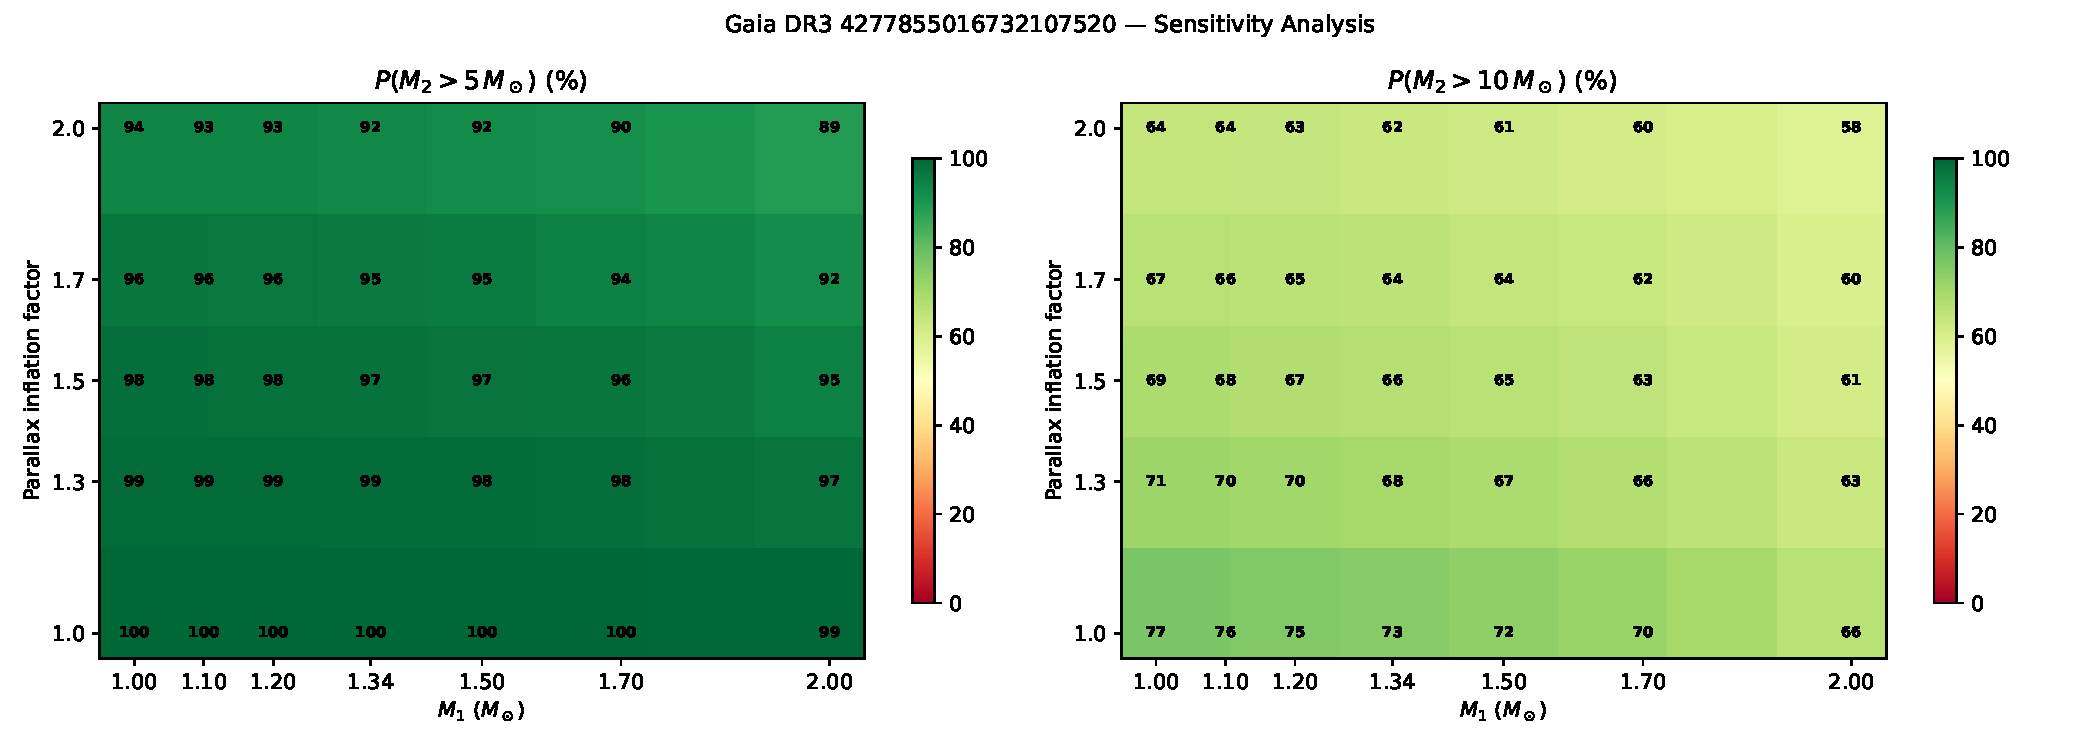
\includegraphics[width=\textwidth]{figures/fig_sensitivity.pdf}
\caption{Sensitivity analysis showing $P(M_2 > 5\,\Msun)$
(\textit{left}) and $P(M_2 > 10\,\Msun)$ (\textit{right}) as a
function of adopted primary mass $M_1$ and parallax-error
inflation factor.  At the fiducial values ($M_1 = 1.34\,\Msun$,
inflation $= 1.7$), $P(M_2 > 5\,\Msun) \approx 95$~per~cent.}
\label{fig:sensitivity}
\end{figure*}

% ====================================================================

\label{lastpage}
\end{document}
